\documentclass[11pt, a4paper]{article}

% === PACKAGES ===
\usepackage{booktabs}
\usepackage{amsfonts}
\usepackage{nicefrac}
\usepackage{microtype}
\usepackage{graphicx}
\usepackage{amsmath, amssymb, amsthm}
\usepackage{natbib}
\usepackage{doi}
\usepackage{hyperref}
\usepackage{listings}
\usepackage{float}
\usepackage{xcolor}
\usepackage{fancyhdr}
\usepackage{subcaption}
\usepackage[nomarkers,notables]{endfloat}

\lstset{
  language=Python,
  basicstyle=\ttfamily\small,
  keywordstyle=\color{blue!70!black},
  commentstyle=\color{gray!70!black},
  stringstyle=\color{orange!80!black},
  showstringspaces=false,
  frame=single,
  numbers=left,
  numberstyle=\tiny,
  numbersep=6pt,
  columns=fullflexible,
  breaklines=true,
  extendedchars=true,
  inputencoding=utf8,
  literate={α}{{\(\alpha\)}}1
           {β}{{\(\beta\)}}1
           {γ}{{\(\gamma\)}}1
           {δ}{{\(\delta\)}}1
           {ε}{{\(\epsilon\)}}1
           {λ}{{\(\lambda\)}}1
           {μ}{{\(\mu\)}}1
           {π}{{\(\pi\)}}1
           {σ}{{\(\sigma\)}}1
           {τ}{{\(\tau\)}}1
           {φ}{{\(\phi\)}}1
           {ψ}{{\(\psi\)}}1
           {∈}{{\(\in\)}}1
           {∑}{{\(\sum\)}}1
           {Σ}{{\(\Sigma\)}}1
           {∏}{{\(\prod\)}}1
           {√}{{\(\sqrt\)}}1
           {ℓ}{{\(\ell\)}}1
           {η}{{\(\eta\)}}1
}

% === MACROS ===
\newtheorem{theorem}{Theorem}
\newtheorem{proposition}{Proposition}
\newtheorem{lemma}{Lemma}
\newtheorem{definition}{Definition}
\theoremstyle{remark}
\newtheorem{remark}{Remark}
\newcommand{\R}{\mathbb{R}}
\newcommand{\E}{\mathbb{E}}

% === CUSTOM FORMULAS ===

\newcommand{\T}{\mathcal{T}}
\newcommand{\Cov}{\mathrm{Cov}}
\newcommand{\ARMA}{\mathrm{ARMA}}
\newcommand{\ARIMA}{\mathrm{ARIMA}}
\newcommand{\AR}{\mathrm{AR}}
\newcommand{\GARCH}{\mathrm{GARCH}}
\newcommand{\ARCH}{\mathrm{ARCH}}
\newcommand{\entFF}[2]{[\![ #1, #2 ]\!]}
\newcommand{\N}{\mathbb{N}}
\newcommand{\code}[1]{\texttt{#1}}
\newcommand{\Z}{\mathbb{Z}}

\begin{document}

\subsection{Framework}

In order to discuss the dynamics of the data based on time-series analysis, let us first explain some notations. Whether it is for french or german energy prices, we'll consider the time space:
\begin{align*}
\T = \{ \mathrm{hour}\!:\!\mathrm{min} \mid \mathrm{hour} \in \entFF{0}{23}, \; \mathrm{min} \in \{0, 15, 30, 45\}\}.
\end{align*}
Every process $X$ considered in this section will take as events the times in the space $\T$, and will span from day $1$ to day $365$, meaning we'll write $(X_t)_t$ instead of $(X_t)_{t \in \entFF{1}{365}}$. Moreover, expectancies will be taken as if the times were chosen uniformly at random in $\T$.

\subsection{Test of stationarity}

\subsubsection{Expectancy function}

In order to modelise our data as $\ARMA(p,q)$ processes, we first need to assess if we can assume the data to be stationary. Let's recall that a process $(X_t)_t$ is said to be (weakly-)stationary if it's square-integrable, its expectancy function is constant and for all $0 \leq s \leq t$, $\Cov(X_s, X_t)$ only depends on $t-s$. To test the last two hypothesis, we need to run the computation of the expectancies and the autocovariance function.

\begin{table}[H]
\centering
\caption{Means and standard deviation of the mean prices per day.}
\label{tab:statio}
\begin{tabular}{lcc}
\toprule
Country & Mean price (€) & Ratio std/mean \\
\midrule
France & 61.08 & 0.32  \\
Germany-Luxembourg  & 89.39 & 0.31 \\
\bottomrule
\end{tabular}
\end{table}
The ratio between standard deviation and the mean helps on showing if the function $t \mapsto \E(X_t)$ is constant or not. Here, the ratio might seem too high. To try to circumvent this issue, we introduce the differentiation operator
\begin{align*}
\nabla \colon X \mapsto (X_t - X_{t-1})_t.
\end{align*}
By applying this operator $d \in \N^*$ times to a process $X$, it removes polynomial tendencies of degree $d-1$. Then, for example the process $\nabla^2 X$ could prove to have its expectancy function constant, and we could then try to modelise it as an $\ARMA$ process. To retrieve the initial process, one may note that:
\[ Y_t = Y_0 + \sum_{i=1}^t (\nabla Y)_t.\]

Figure \ref{fig:ratio_fr} shows the ratio between standard deviation and mean on the function $t \mapsto \E((\nabla^dX)_t)$ for $d$ varying from $0$ to $100$, while figure \ref{fig:ratio_de} shows the same for Germany. One may notice that the two best ratios are obtained for $d=0$ and $d=1$, meaning we'll be modelising one of the two as an $\ARMA$ process. The next step is to compute the autocovariance function.

\begin{figure}[H]
    \centering
    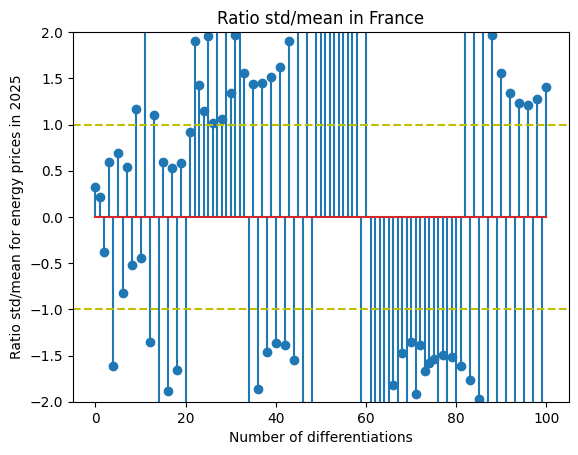
\includegraphics[width=0.58\textwidth]{ratio_fr.png}
    \caption{Ratio std/mean of the expectancy function for the french prices process differentiated $n$ times.}
    \label{fig:ratio_fr}
\end{figure}

\begin{figure}[H]
    \centering
    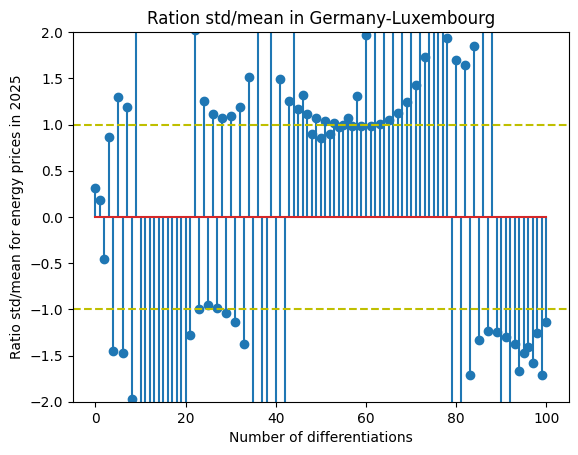
\includegraphics[width=0.58\textwidth]{ratio_de.png}
    \caption{Ratio std/mean of the expectancy function for the german prices process differentiated $n$ times.}
    \label{fig:ratio_de}
\end{figure}

\subsubsection{Autocovariance function}

For a stationary process, computing the autocovariance function is fairly easy. One only needs to compute:

\[ \gamma(n) = \Cov(X_n, X_0), \quad \text{ for every } n \in \N.\]
However, to test the stationarity, we'll be computing for every $n \in \N$,
\[ t \mapsto \Cov(X_{t+n}, X_t),\]
to test whether it is constant or not. We did this computation, and checked the mean and the standard deviation, to figure out which trajectory would be best. Figure \ref{fig:cov_fr} shows the ratio between standard deviation and mean for the autocovariance function, while figure \ref{fig:cov_de} shows the same for Germany. The trajectories depend on the number of times the process has been differentiated. It clearly shows that the best candidate to be modelised as an $\ARMA$ is the energy prices process itself.

\begin{figure}[H]
    \centering
    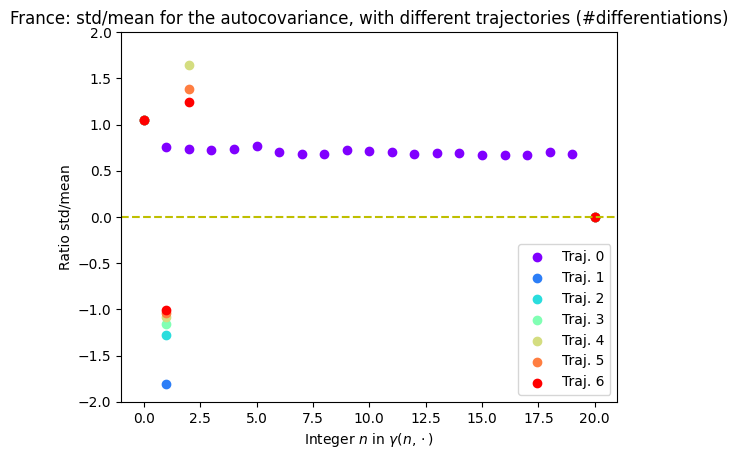
\includegraphics[width=0.58\textwidth]{cov_fr.png}
    \caption{Ratio std/mean of the autocovariance function for the french prices process, with trajectories depending on the number of differentiations.}
    \label{fig:cov_fr}
\end{figure}

\begin{figure}[H]
    \centering
    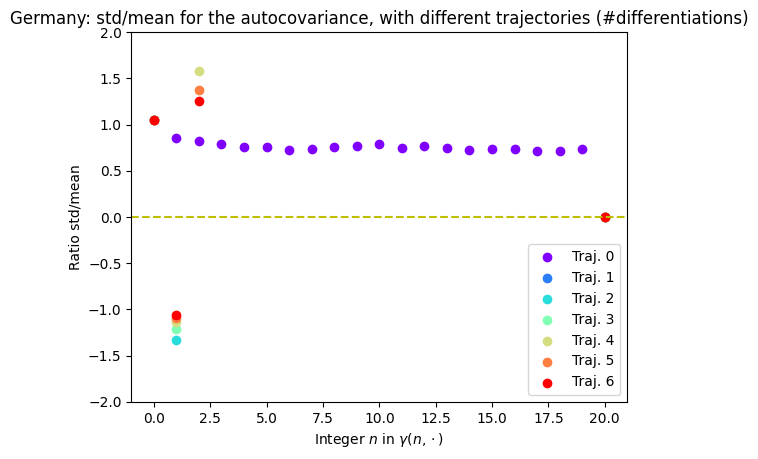
\includegraphics[width=0.58\textwidth]{cov_de.png}
    \caption{Ratio std/mean of the autocovariance function for the german prices process, with trajectories depending on the number of differentiations.}
    \label{fig:cov_de}
\end{figure}

\subsection{ARMA modelisation}

\subsubsection{With statsmodels}

The module \code{statsmodels} is built in Python and provides classes and functions for the estimation of many different statistical models, as well as for conducting statistical tests, and statistical data exploration. In particular, it comes with the extremely useful \code{tsa.arma} function which computes the best fitting ARMA model, given values of $p$ and $q$, minimizing the Akaike information criterion (AIC). This criterion is computed according to this formula:
\[ \mathrm{AIC} = 2N - 2 \ln(L),\]
where $N$ is the number of estimated parameters and $L$ is the maximum of the likelihood function. Given the computation complexity of this function, we ran it over the tuples in $\entFF{0}{5}^2$ to get the best fitting model. Results can be seen in figure \ref{fig:arma_fr} for the french prices, and figure \ref{fig:arma_de} for german prices.

\begin{figure}[H]
    \centering
    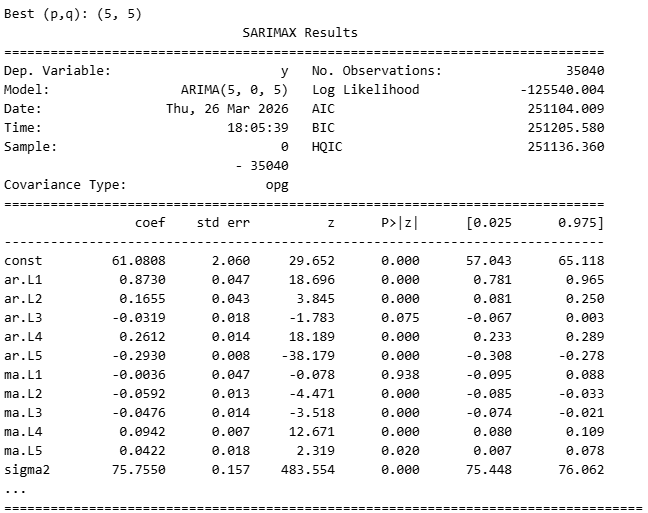
\includegraphics[width=0.58\textwidth]{ARMA.png}
    \caption{Results for the ARMA function of the \code{statsmodels} module (french prices).}
    \label{fig:arma_fr}
\end{figure}

\begin{figure}[H]
    \centering
    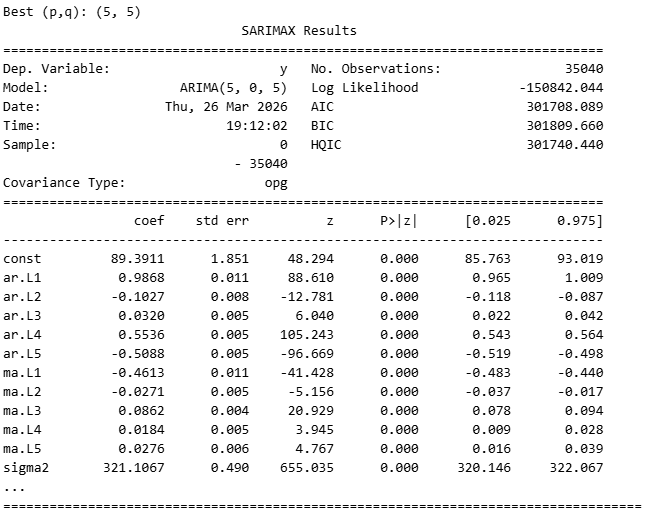
\includegraphics[width=0.58\textwidth]{ARMA2.png}
    \caption{Results for the ARMA function of the \code{statsmodels} module (german prices).}
    \label{fig:arma_de}
\end{figure}

\subsubsection{With an AR(p) process}

An $\AR(p)$ process is an $\ARMA(p,q)$ process in which we let $q = 0$. In this subsection, we try to find an $\AR$ model which could perform better that the $\ARMA(5,5)$ previously found with the \code{statsmodels} module. Suppose we have a process $X$ being $\AR(p)$ with $p \in \N$. Then we can write
\begin{align*}
X_t = \sum_{i=1}^p \phi_i X_{t-i} + \epsilon_t,
\end{align*}
where $\epsilon$ is a white noise of standard deviation $\sigma$. We denote by $\gamma$ the autocovariance function. Then, for all $m \in \N$,
\begin{align*}
\E(X_t X_{t-m}) & = \sum_{i=1}^p \phi_i \E(X_{t-m} X_{t-i}) + \E(\epsilon_t X_{t-m}) \\
\gamma_m & = \sum_{i=1}^p \phi_i \gamma_{m-i} + \sigma^2 \delta_{m, 0},
\end{align*}
by definition of $\gamma$ and using the result in the course for the second term. These equations are known as Yule-Walker equations. Now, let us consider the sequence of matrices defined by
\begin{align*}
\Gamma_m = \begin{pmatrix}
\gamma_0 & \gamma_{-1} & \cdots & \gamma_{1-m} \\
\gamma_1 & \ddots & & \vdots \\
\vdots & & \ddots & \vdots \\
\gamma_{m-1} & \cdots & \cdots & \gamma_0
\end{pmatrix}, \quad \text{ for all } m \in \N.
\end{align*}
Then, one gets from the Yule-Walker equations that for every $m \in \N^*$,
\begin{align*}
\begin{pmatrix}
\gamma_1 & \cdots & \gamma_m
\end{pmatrix}^T = \Gamma_m \begin{pmatrix}
\phi_1 & \cdots & \phi_m
\end{pmatrix}^T.
\end{align*}
Assuming $\Gamma_m$ is invertible:
\begin{align*}
\begin{pmatrix}
\phi_1 & \cdots & \phi_m
\end{pmatrix}^T = \Gamma_m^{-1} \begin{pmatrix}
\gamma_1 & \cdots & \gamma_m
\end{pmatrix}^T.
\end{align*}
Then we get, for $m=0$,
\begin{align*}
\sigma^2 = \gamma_0 - \sum_{i=1}^p \phi_i \gamma_{-i}.
\end{align*}
We can use that $\gamma_n = \gamma_{-n}$ for every $n \in \Z$. Then we compute the $\mathrm{AIC}$ for each model $p$, using that we estimated $N = p + 1$ parameters, i.e.:
\begin{align*}
\mathrm{AIC}_p = 2(p+1) + (T-p) \ln(\sigma^2) + (T-p)(1 + \ln(2\pi)),
\end{align*}
here $T = 365$ (number of days in a year, sample size), and we substract $p$ because the first $p$ observations are fixed. Figure \ref{fig:aic_fr} shows the results for french prices, while figure \ref{fig:aic_de} shows the results for german prices. It is clear that the $\AR$ model is better with increasing $p$. However, we cannot compare the values of AIC between this computation and the one of \code{statsmodels} module, because they may differ from a constant.

\begin{figure}[H]
    \centering
    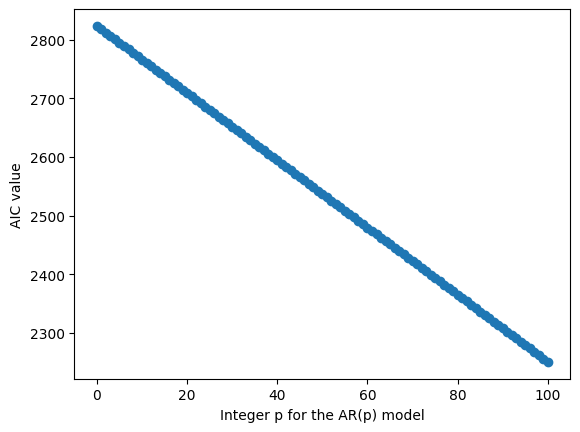
\includegraphics[width=0.58\textwidth]{aic_fr.png}
    \caption{Results for the AIC function for french prices.}
    \label{fig:aic_fr}
\end{figure}

\begin{figure}[H]
    \centering
    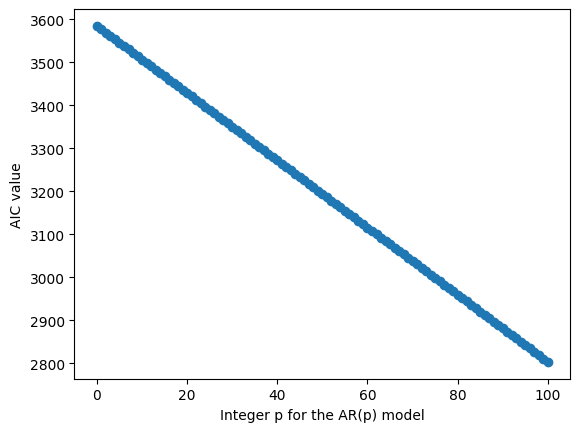
\includegraphics[width=0.58\textwidth]{aic_de.png}
    \caption{Results for the AIC function for german prices.}
    \label{fig:aic_de}
\end{figure}

To check whether our results are compatible with \code{statsmodels}, we ran the code over the best fitting AR model for $p$ varying from $0$ to $25$. Figure \ref{fig:ar_fr} shows the results for french prices, while figure \ref{fig:ar_de} show the results for german prices. In both cases, the best model is $\AR(25)$, which is compatible with the two graphs obtained with the Yule-Walker equations. Secondly, it's interesting to note that:
\begin{align*}
\mathrm{AIC}(\AR(25)) < \mathrm{AIC}(\ARMA(5,5))
\end{align*}
for french prices, as well as german prices. However, even though we ran the tests over $25$ values of $p$, instead of $36$ values of $(p,q)$, the code took $50\%$ more time to compile. Thus, it should be best to use ARMA modelisation rather than AR, especially for large values of $p$, and one can use Yule-Walker equations to get a faster result.

\begin{figure}[H]
    \centering
    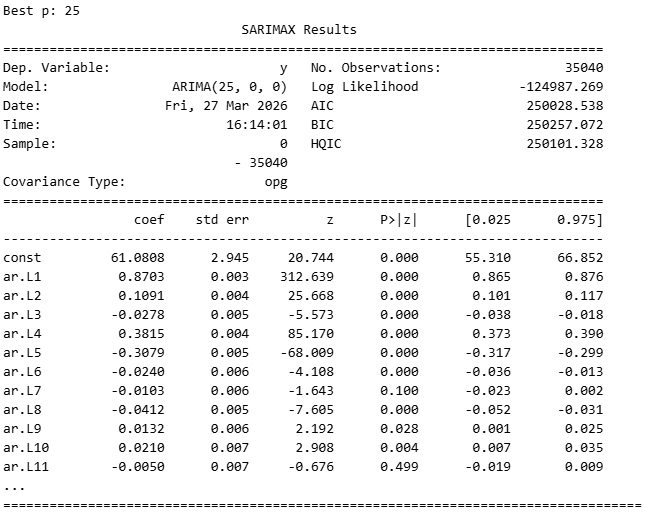
\includegraphics[width=0.58\textwidth]{ar_fr.png}
    \caption{Results for the AR modelisation with the \code{statsmodels} module for french prices.}
    \label{fig:ar_fr}
\end{figure}

\begin{figure}[H]
    \centering
    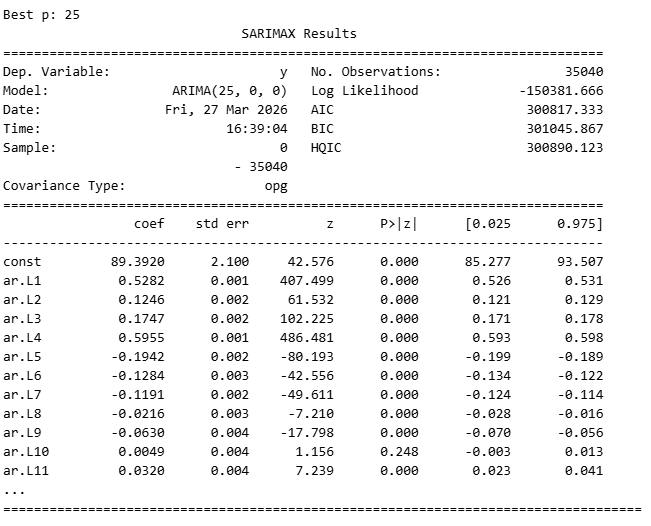
\includegraphics[width=0.58\textwidth]{ar_de.png}
    \caption{Results for the AR modelisation with the \code{statsmodels} module for french prices.}
    \label{fig:ar_de}
\end{figure}

\subsection{GARCH modelisation}

As the data processed consists of prices, one may argue that ARMA modelisation is not adapted, and that we need to modelise it by a GARCH model. This section quickly explores this case. We used the library \code{arch} to implement this.

Figures \ref{fig:garch11_fr} and \ref{fig:garch11_f_fr} show the fitting of a $\GARCH(1,1)$ model on the french prices, with the prices on each day being averaged. Then, the model predicts what could happen in the next month. Seeing the graphs, it seems that modelising the prices as a GARCH is much more interesting that an ARMA, as our data isn't clearly stationary in the first case. In addition, finding a linear invertible transform that can make the data stationary is hard. In GARCH case, the fitting is believable, even though that's not nearly the case for the forecasting.

\begin{figure}[H]
    \centering
    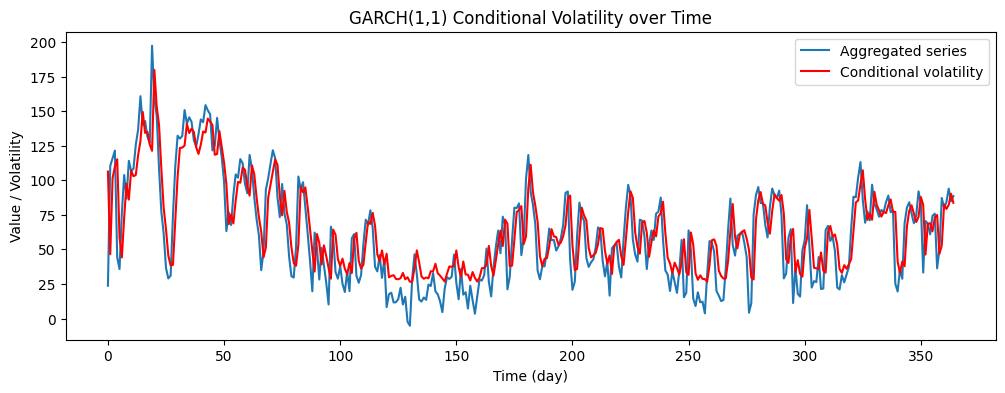
\includegraphics[width=0.58\textwidth]{garch11_fr.png}
    \caption{GARCH(1,1) modelisation for french prices.}
    \label{fig:garch11_fr}
\end{figure}

\begin{figure}[H]
    \centering
    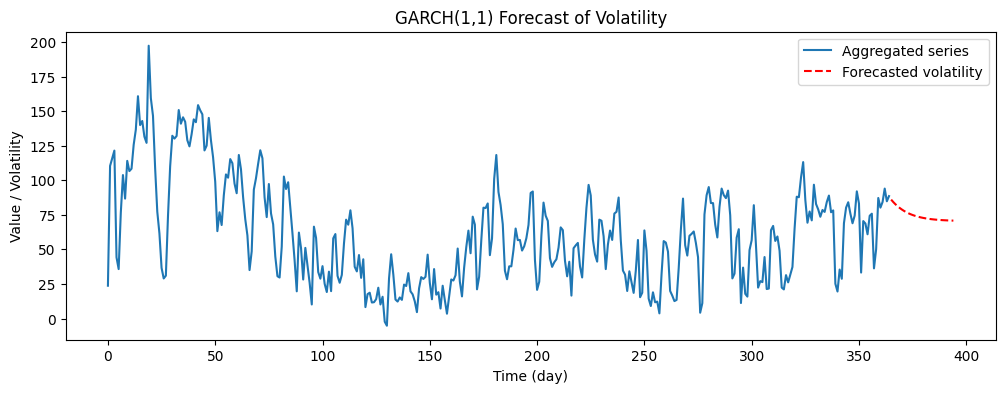
\includegraphics[width=0.58\textwidth]{garch11_f_fr.png}
    \caption{GARCH(1,1) forecast for french prices.}
    \label{fig:garch11_f_fr}
\end{figure}

Figures \ref{fig:garch22_fr} and \ref{fig:garch22_f_fr} show the fitting of a $\GARCH(2,2)$ model on the french prices ; while figures \ref{fig:garch1010_fr} and \ref{fig:garch1010_f_fr} show the fitting of a $\GARCH(10,10)$ model on the french prices. We see that both models $\GARCH(2,2)$ and $\GARCH(10, 10)$ act nearly similarly on the french prices. However, the forecastings differ completely. On one hand, $\GARCH(2,2)$ predicts a drop in the prices which seems linear, contrary to the prediction of a quadratic drop with $\GARCH(1,1)$. On the other hand, $\GARCH(10,10)$ seems to be predicting the average of the time-series we analysed. As the processes act as white noises, it's not surprising to see the forecast converging to a constant value.

\begin{figure}[H]
    \centering
    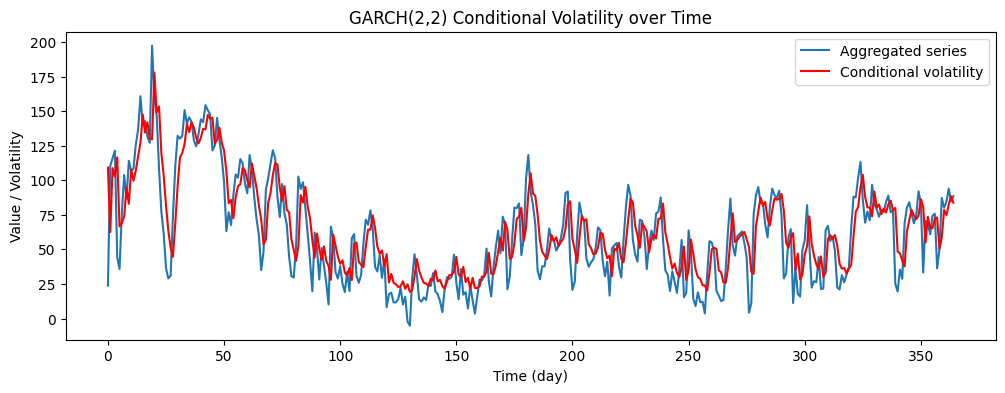
\includegraphics[width=0.58\textwidth]{garch22_fr.png}
    \caption{GARCH(2,2) modelisation for french prices.}
    \label{fig:garch22_fr}
\end{figure}

\begin{figure}[H]
    \centering
    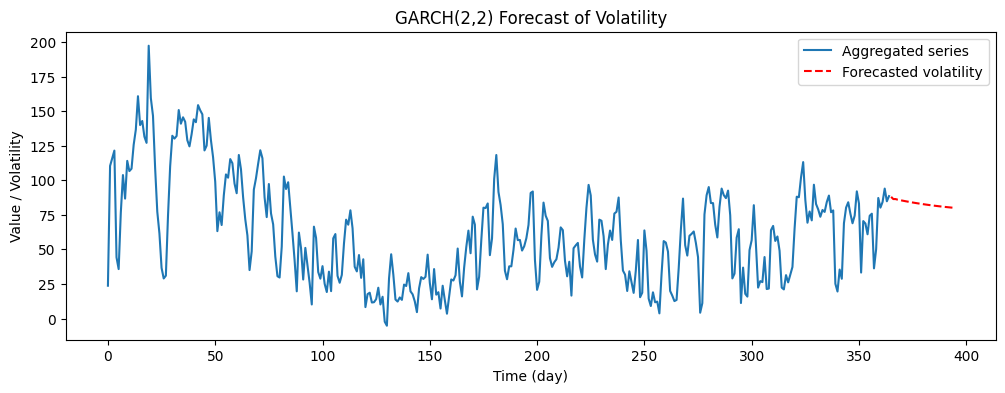
\includegraphics[width=0.58\textwidth]{garch22_f_fr.png}
    \caption{GARCH(2,2) forecast for french prices.}
    \label{fig:garch22_f_fr}
\end{figure}

\begin{figure}[H]
    \centering
    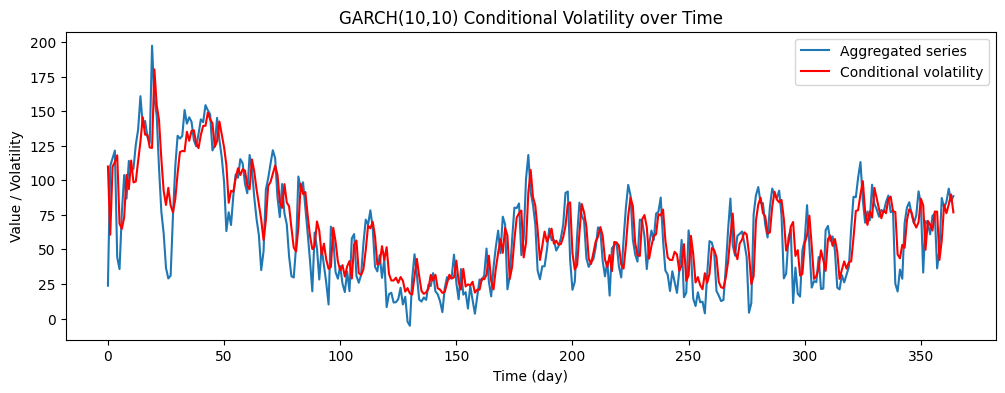
\includegraphics[width=0.58\textwidth]{garch1010_fr.png}
    \caption{GARCH(10,10) modelisation for french prices.}
    \label{fig:garch1010_fr}
\end{figure}

\begin{figure}[H]
    \centering
    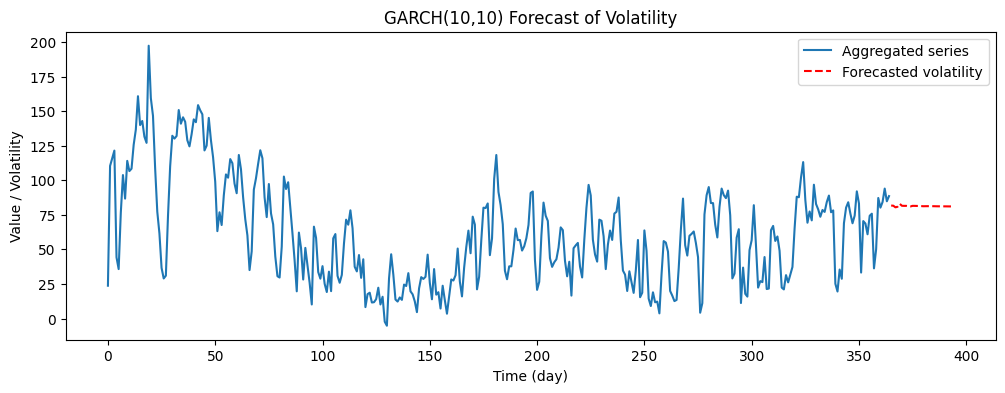
\includegraphics[width=0.58\textwidth]{garch1010_f_fr.png}
    \caption{GARCH(10,10) forecast for french prices.}
    \label{fig:garch1010_f_fr}
\end{figure}

Thus, in our case, the french and german energy prices might be better off modelised by a GARCH model, which is in agreement with the course we took: financial time series are not compatible with ARMA processes, that's why GARCH processes were invented in the first place.

\end{document}